\section{Installing Uintah} \label{Sec:installation}

The Uintah library is composed of several executables and a generic
library framework for solving PDEs on structured AMR grids.  The VisIt
and Teem libraries are used to visualize the resulting data.

Uintah can be obtained either from a tarball \tt
http://www.uintah.utah.edu \normalfont or by using svn to download the
latest source from the following:

\begin{Verbatim}[fontsize=\footnotesize]
  svn co https://code.sci.utah.edu/svn/SCIRun/trunk Uintah
\end{Verbatim}

The above command checks out the Uintah source tree and installs it
into a directory called Uintah in the users home directory.

VisIt can be obtained from https://wci.llnl.gov/codes/visit/. And Teem
can be obtained from http://teem.sourceforge.net/.

\subsection{Library Dependencies}

Uintah depends on several different libraries that are commonly
available or easily installable on various Linux or Unix like OS
distributions.  

Required libraries:

mpi (openmpi, mpich, or lam or a vendor supplied mpi library)
blas
lapack
make
libxml2-devel
zlib-devel
c++
subversion
ccmake

Useful libraries:
hypre-2.0
petsc 2.3.3

Hypre 2.0 can be downloaded from
https://computation.llnl.gov/casc/hypre/software.html.

Petsc 2.3.3 can be downloaded from
http://www.mcs.anl.gov/petsc/petsc-as/download/index.html.

\subsection{Debian Dependencies}

The Debian OS offers the vast majority of libraries necessary for
installing Uintah with the exception of VisIt and Teem.

Installing the following libraries will ensure that all dependencies
required for Uintah are satisfied: subversion libhypre-dev petsc-dev
libxml2-dev zlib1g-dev liblapack-dev cmake cmake-curses-gui.

Once these libraries are installed, Teem and VisIt can be installed
followed by installation of Uintah.

\subsection{Fedora Core 9 Dependencies}

Fedora Core 9 offers all the dependencies except for petsc and hypre.
Installation of the following libraries: openmpi-devel openmpi-libs
lapack-devel gcc-gfortran blas-devel gcc-c++ libxml2-devel subversion
make tar diffutils.

\subsection{CentOS 5 Dependencies}

CentOS 5 does not provide an openmpi rpm, however a src.rpm can be
downloaded from http://www.open-mpi.org:80/software/ompi/v1.3/ and
installed via rpmbuild

\begin{Verbatim}
rpmbuild --rebuild --define 'dist .centos5' openmpi-1.3.1-1.src.rpm
rpm -i openmpi-1.3.1-1.*.rpm
\end{Verbatim}

The location of the rpm is likely to be found in
/usr/src/redhat/RPMS/ARCH where ARCH is either i386 or x86\_64.

Once mpi has been built, the other libraries can be installed:
lapack-devel gcc-gfortran blas-devel gcc-c++ libxml2-devel subversion
make tar diffutils.

\subsection{MPI issues}

The openmpi library that is installed with Fedora Core 9 needs to have
a 'helper' directory set up with symbolic links assigned so that
Uintah can find the location of specific include files and shared
libraries.

Execute the following as root:

\begin{Verbatim}

mkdir /usr/local/openmpi
cd /usr/local/openmpi
ln -s /usr/include/openmpi/1.2.4-gcc include
ln -s /usr/lib64/openmpi/1.2.4-gcc lib

\end{Verbatim}



\subsection{Petsc Installation}

Petsc can be installed by executing the following simplified
instructions.  Please refer to the petsc website for comprehensive
installation instructions if you encounter any difficulties.

Download petsc-2.3.3 from
http://www.mcs.anl.gov/petsc/petsc-as/download/index.html

The following configure script assumes the location of mpi is in
/usr/local/openmpi using the Fedora Core 9 OS.  For other OS
distributions, the location of the mpi libraries may be found
automatically.

\begin{Verbatim}
  
tar zxf petsc-2.3.3.tar.gz
cd petsc-2.3.3-p15

./config/configure.py --with-shared --with-debugging=0 --with-mpi-dir=/usr/local/openmpi/ --prefix=/usr/local/petsc

make all

make install

\end{Verbatim}

\subsection{Hypre Installation}

Hypre can be installed by executing the following simplified
instructions, however, if you encounter problems please refer to the
hypre website for troubleshooting.

Download hypre-2.0 from
https://computation.llnl.gov/casc/hypre/download/hypre-2.0.0\_reg.html

If installing hypre on a 64bit platform, hypre must be modified to add
the -fPIC compile option.  After unpacking the hypre tar file, edit
the Makefile in hypre-2.0.0/src/lapack and add the -fPIC to line 128.
It should look like the following:

\begin{verbatim}

${CC} -c -fPIC dlamch.c

\end{verbatim}

Depending on the location of the mpi libraries, i.e. location of mpi.h
and libmpi.so, the configure line for hypre should look something like this:

\begin{Verbatim}

cd hypre-2.0.0/src

./configure --enable-shared
--with-MPI-include=/usr/local/openmpi/include/
--with-MPI-lib-dirs=/usr/local/openmpi/lib/ --with-MPI-libs="mpi pmpi
util" --prefix=/usr/local/ CFLAGS=-DMPIPP_H CXXFLAGS=-DMPIPP_H

make

make install

\end{Verbatim}

 

\subsection{Teem Installation}
\label{sec:teem}


Download Teem from http://teem.sourceforge.net/download/index.html.  Teem uses cmake to configure the build system. Installation instructions for Teem are found at http://teem.sourceforge.net/build.html.  Simplified instructions are as follows:

\begin{verbatim}

tar zxf teem-1.10.0-src.tar.gz

cd teem-1.10.0-src/

mkdir teem-build

cd teem-build

ccmake ../

Teem and VisIt need to be installed first before Uintah can be configured.

Use the arrow keys to scroll down to the fourth line 'BUILD_SHARED_LIBS' and press the 
return key to toggle the 'ON' flag.

Press the 'c' key

Press the 'g' key

make

make install

\end{verbatim}

The Teem libraries and include files will be install in /usr/local hierarchy.

\subsection{VisIt Installation}

\subsubsection{Client/ Server}
\label{sec:ClientServer}

You would most likely will want to install a VisIt server on a multiprocessor machine. This requires you to build the server from source (as it is needed to compile the UDA reading plugin). You can then install any client on your local machine and attach to the server. 

\subsubsection{Prebuilt binaries}
\label{sec:PrebuiltBinaries}

If you have a system that matches the prebuilt binaries, found at \url{https://wci.llnl.gov/codes/visit/executables.html}, you may want to try one. In most cases you will want to build your own binaries. There are currently no universal binaries available for Mac OS X 10.5 (leopard).

\subsubsection{Using the build script}
\label{sec:UsingTheBuildScript}

We recommend that you first try the visit build script (WARNING, make sure you get the must recent version of this script. The build script must correspond to the version of VisIt you wish to install. The latest version is 1.11.2). This is a link to the script, \url{https://wci.llnl.gov/codes/visit/1.11.2/build\_visit}.

You can also use the following command on the terminal (from most linux boxes), to download the file directly, 

\begin{Verbatim}[fontsize=\footnotesize]
wget https://wci.llnl.gov/codes/visit/1.11.1/build_visit
chmod +x build_visit
\end{Verbatim}

\normalfont The chmod is used to set execute permissions on the file.

build\_visit is a bash build script that downloads and builds VisIt as well as all of the necessary third party libraries. The script makes use of the dialog program which allows you to customize your build.

Once you have the script, you would need to execute the following on the terminal,

\begin{Verbatim}[fontsize=\footnotesize]
./build_visit --makeflags '-j#'
\end{Verbatim}
	
\normalfont where '\#' is the number of processors to use, while building VisIt. 

This would launch a dialog window and would require you to select some options (using the Space bar). You should select the 'Parallel' option, if you wish to have a parallel build of the engine. Once you have selected the parallel option, you may be required to specify the path to the include and lib directories of your MPI installation. 

The process of building VisIt may be slow and it may appear that nothing is happening. To verify the build script is not hanging, open another terminal and tail the file build\_visit\_log	. 

\begin{Verbatim}[fontsize=\footnotesize]
tail -f build_visit_log
\end{Verbatim}

\normalfont  
\subsubsection{Parallel OS X build}
\label{sec:ParallelOSXBuild}

A full parallel OS X build can be built using the instructions above, but it will fail when it tries to build the visit executable (the last stage of the script). When it fails, you will need to follow the instructions for building in parallel on a Mac. 

\begin{Verbatim}[fontsize=\footnotesize]
http://visitusers.org/index.php?title=Building_in_parallel_on_a_Mac
\end{Verbatim}
  
Note particularly the changes that need to be made in the file, 

\begin{Verbatim}[fontsize=\footnotesize]
<path\_to\_visit>/visit1.11.2/src/config-site/<your_machine_name>.conf
\end{Verbatim}

\normalfont Once you make these edit's, you can then finish building VisIt by typing make in the \tt <path\_to\_visit>/visit1.11.2/src \normalfont directory.  

\subsubsection{When the build script fails}
\label{sec:WhenTheBuildsSriptFails}

Sometimes the build script doesn't work depending on your installation. When this happens, you may be forced to build everything by hand. The instructions for doing this are carefully outlined in the VisIt Build Notes file, 

\begin{Verbatim}[fontsize=\footnotesize]
https://wci.llnl.gov/codes/visit/1.11.2/BUILD_NOTES
\end{Verbatim}

\subsubsection{VisIt executable}
\label{sec:VisItExecutable}

After a successful build, the executable will be placed in,

\begin{Verbatim}[fontsize=\footnotesize]
<path\to\visit>/visit1.11.2/src/bin
\end{Verbatim}

\subsubsection{Building and installing the UDA reader plugin}
\label{sec:BuildingAndInstallingUDAPlugin}

Add the following arguements to the Uintah configure line,

\begin{Verbatim}[fontsize=\footnotesize]
--with-visit=/path/to/visit 
--with-teem=/path/to/teem
\end{Verbatim}

For example,

\begin{Verbatim}[fontsize=\footnotesize]
--with-teem=/usr/sci/projects/Manta/Thirdparty/Linux/gcc-4.1.2-64bit/teem \
--with-visit=/home/csafe/dav/VisIt/blaze/visit1.11.2 \
\end{Verbatim}

Note, the \tt visit1.11.2 \normalfont directory you point at should have \tt data\normalfont , and \tt src \normalfont sub-directories; and the \tt teem \normalfont directory should have \tt bin\normalfont , \tt include\normalfont , and \tt lib \normalfont sub-directories.

\subsubsection{How it works}
By specifying the above configure arguments (to the Uintah configure), Uintah will automatically build a VisIt plugin (when you type "make"). The plugin will be placed in (a sub-directory of) ~/.visit. When VisIt is run, it will find the plugin and allow for reading UDA's.

\subsubsection{Remote visualization}
In order to read data on a remote machine, you will need to have a version of VisIt and the UDA reader plugin installed on that machine. You will also need to make sure that the VisIt executable is in your path. You may need to edit your shell's .rc file so that the path to VisIt is included in your shell's PATH variable.

NOTE: The version of VisIt installed on your local desktop and the remote machine should be the same.

\paragraph{Host Profile}
Next you will want to set up a Host Profile for your remote machine. Select 'Host Profiles' from the 'Options' menu and set up a new profile as shown in figure ~\ref{VisItHostProfile}.

\begin{figure}
  \center
  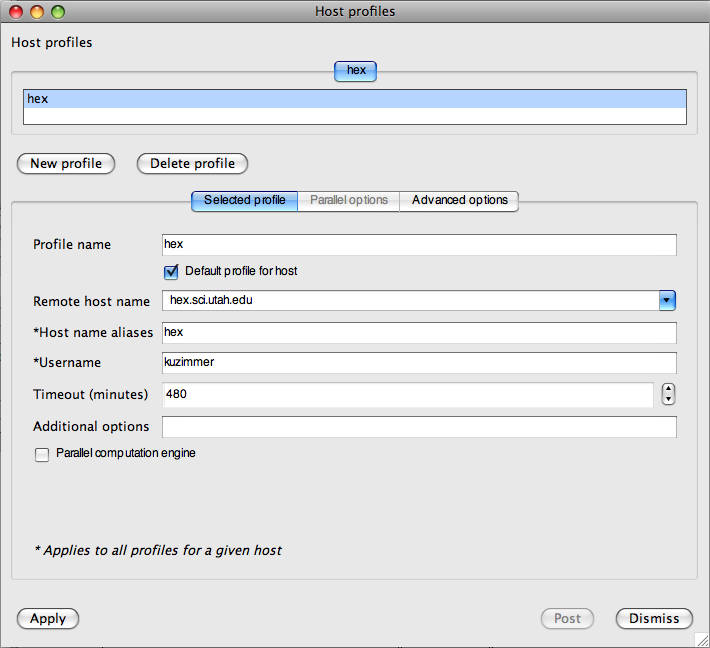
\includegraphics[scale=0.5]{VisItHostProfile.png}
  \caption{Setting up Host Profile}
  \label{VisItHostProfile}
\end{figure}

After filling in the remote machine information, select the 'Advanced options' tab, then 'Networking' and check the 'Tunnel data connections through SSH' option. This is illustrated in figure~\ref{VisItHostProfileAdv}. Click on 'Apply' and then do a 'Save Settings' in the 'Options' menu on the gui.

\begin{figure}
  \center
  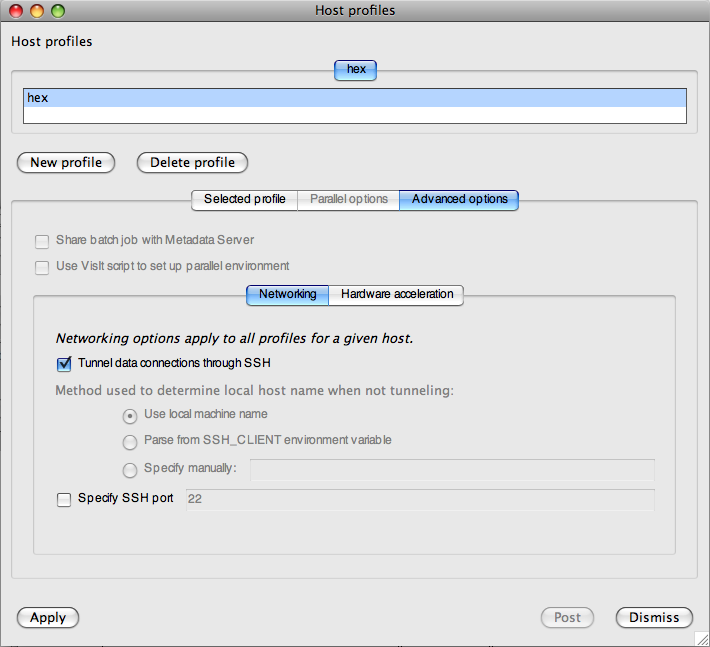
\includegraphics[scale=0.5]{VisItHostProfileAdv.png}
  \caption{Setting up advanced options}
  \label{VisItHostProfileAdv}
\end{figure}

For the remote visualization option to work, you must have ports 5600 - 5609 open. You can try this by running the following on your local desktop (on linux distributions),

\begin{Verbatim}[fontsize=\footnotesize]
traceroute -p 560[0-9] <remote machine> 
\end{Verbatim}

If the tunneling option doesn't works, try the option as shown in figure~\ref{VisItHostProfileAdv2}.

\begin{figure}
  \center
  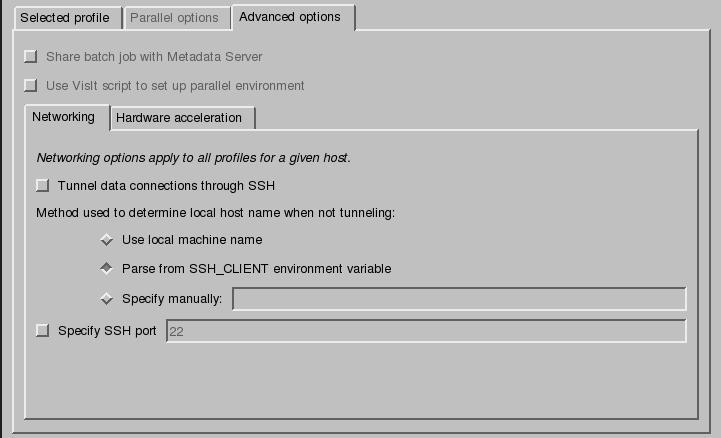
\includegraphics[scale=0.5]{VisItHostProfileAdv2.png}
  \caption{Setting up advanced options}
  \label{VisItHostProfileAdv2}
\end{figure}

Now you should be able select 'Open' from VisIt's 'File' menu. After selecting your host from the host entry list, you will be prompted for a password on the remote machine (unless you have set up passwordless ssh access). 

Once the ssh login has completed, you should see the directory listing. You can then change directories to your UDA and load the data. 

%VisIt has a build script which builds VisIt plus all of its dependencies.

%The build script can be downloaded from
%https://wci.llnl.gov/codes/visit/1.11.2/build\_visit

%Make the build\_script executable:

%\begin{verbatim}

%chmod +x build\_script

%\end{verbatim}

%Create a directory for VisIt and launch the build\_script using four
%processors (-j4):

%\begin{verbatim}

%mkdir Visit

%cp build\_script Visit

%cd Visit

%./build\_script --makeflags '-j4'

%\end{verbatim}

%The build\_visit script will launch a GUI.  Use the space key to
%unselect the Optional and then scroll down to the Parallel option and
%select that.  The GUI will determine the location of the mpi libraries
%and then start the build process.  All source files will be downloaded
%and installed in the ~/Visit/visit1.11.2 directory.  The \tt visit
%\normalfont executable is found in ~/Visit/visit1.11.2/src/bin .

\subsubsection{Configuring Uintah}

cd to\tt ~/Uintah \normalfont and create the following directories:
dbg and opt

\begin{verbatim}
mkdir dbg opt
\end{verbatim}

Go to the dbg directory and enter the following:

\begin{Verbatim}[fontsize=\footnotesize]
../src/configure --enable-debug --with-teem=/usr/local
--with-visit=/home/user_name/Visit/visit1.11.2
\end{Verbatim}

If building on a 64bit platform, append \tt --enable-64bit \normalfont
to the configure line.

After the configuration process, type \tt make \normalfont to compile
Uintah.

Once a debug build has finished, change to the opt directory and enter
the following configure line:

\begin{Verbatim}[fontsize=\footnotesize]
./src/configure --enable-optimze --enable-assertion-level=0 
--with-teem=/usr/local
--with-visit=/home/user_name/Visit/visit1.11.2
\end{Verbatim}

Then build the software by typing \tt make \normalfont at the command line.

\subsection{Installing Visualization Software}

Visualization of Uintah data is currently possible using any of three
software packages.  These are SCIRun, VisIt and Manta.  Of these, SCIRun is
no longer supported, although legacy versions will continue to work.  The
VisIt package from LLNL is general purpose visualization software that offers
all of the usual capabilities for rendering scientific data.  It is still
developed and maintained by LLNL staff, and its interface to Uintah data is
supported by the Uintah team.  Manta offers volume rendering and particle
visualizaton based on parallel (shared memory) ray tracing techniques.
While the capabilities of Manta are more limited, it is a fast way to
interactively interrogate reasonably large datasets, provided the user has
access to a reasonable shared memory resource, (e.g. an 8 core desktop system).

\subsection{Installing Manta C-SAFE Scene}

\subsection{Building Manta}

For complete build instructions for Manta, please refer to
http://software.sci.utah.edu/manta/index.php/CSAFE.  

\begin{enumerate}
\item
Install Teem \ref{sec:teem}.
\item
Install wxPython 2.8+ http://www.wxpython.org/ .  
to verify that you have 2.8+ installed, run
\begin{Verbatim}
> python
>>> import wxversion
>>> wxversion.getInstalled()
['2.8-mac-unicode']
\end{Verbatim}
\item
The next step is to download the Manta source and create a build directory.
\begin{Verbatim}
mkdir Manta
mkdir Manta/build
svn co https://code.sci.utah.edu/svn/Manta/trunk Manta/src
\end{Verbatim}
\item
The build is configured with cmake.
\begin{Verbatim}
cd Manta/build
ccmake ..
\end{Verbatim}
\item
 First you will need to set the TEEM library path. Press the down arrow until you get to the variable FOUND\_TEEM\_BIN. Set this to the location of your TEEM installation by pressing enter and entering the path, eg /usr/bin. Press "c" to configure. If you get errors about not finding TeemConfig.cmake (in older versions before Nov. 2008 it was called TEEMConfig.cmake), you can manually set this by pressing t and going down to the variable named FOUND\_TEEMCONFIG\_CMAKE and setting it to TeemConfig.cmake from your TEEM installation. 
 \item
 You will need to enable the following by scrolling down to them and pressing "enter" if they do not already say ON: BUILD\_SWIG\_INTERFACE, BUILD\_NRRDPARTICLES, MANTA\_SSE. Now press "c" to configure. 
 \item
 You should now see an option called SCENE\_CSAFE, enable this if not already. Now press "c" to configure again. 
 \item
 Click "g" to generate the cmake files. you can now build Manta again by typing make. 
\end{enumerate}

\subsection{Running Manta}

To run the C-SAFE scene: 
\begin{Verbatim}
  Manta/build/bin/csafe_scene
\end{Verbatim}

The csafescene window will open showing a transfer function editor.  To add files to load run:
\begin{Verbatim}
  File -> Add/Remove NRRD Files
\end{Verbatim}

\begin{figure}[thb!]
  \center
  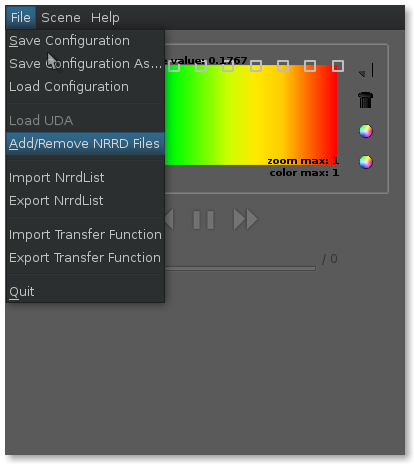
\includegraphics[width=.48\linewidth]{manta_files.png}
  \caption{Opening the scene}
  \label{fig:manta_files}
\end{figure}

This will open a window where you can add volume and particle files in .nrrd or .nhdr formats.  Select add particle file(s) and open a particle nrrd file in .nhdr or .nrrd format.  These nrrd files should be created with the uda2nrrd tool.

\begin{figure}[thb!]
  \center
  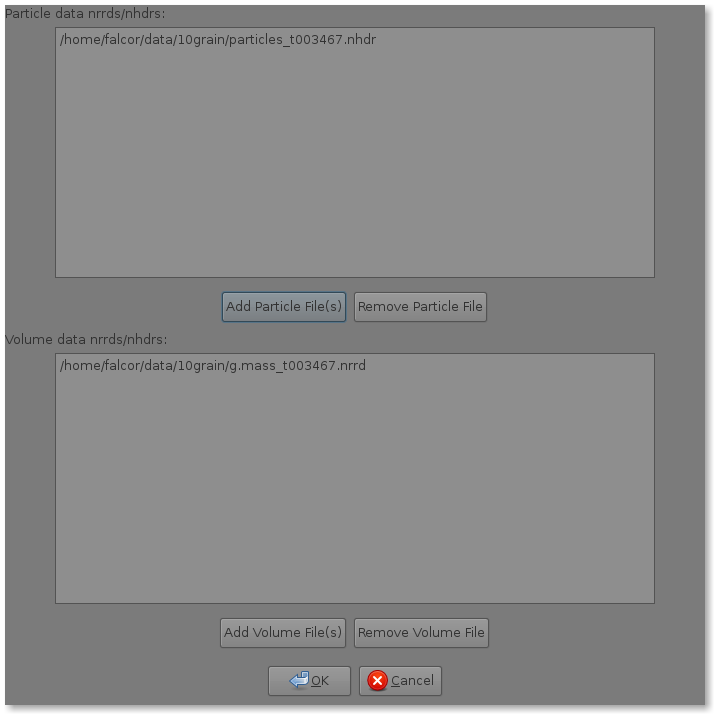
\includegraphics[width=.48\linewidth]{manta_add_files.png}
  \caption{Adding files to the scene}
  \label{fig:manta_add_files}
\end{figure}

A similarly named volume nrrd should be automatically added if in the same folder.  Close the window by pressing "OK".  The files won't be loaded yet so you can make modifications to the data to be loaded in before loading them.  To load the files:

\begin{Verbatim}
  Scene -> Generate
\end{Verbatim}

The resulting csafescene window should look similar to:

\begin{figure}[thb!]
  \center
  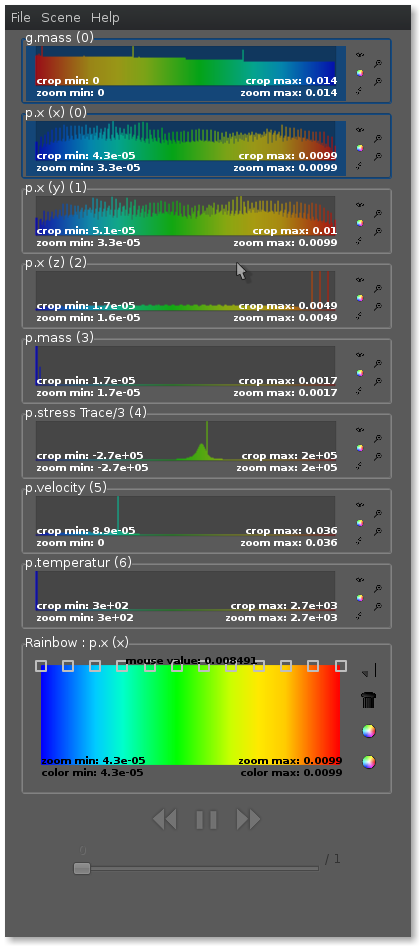
\includegraphics[width=.48\linewidth]{manta_histograms.png}
  \caption{C-SAFE window with histograms from loaded nrrd files}
  \label{fig:manta_histograms}
\end{figure}